\documentclass[a4paper,12pt]{report} %poner [twoside, 12pt] si lo vamos a imprimir

%-----------------------------------------|PAQUETES|-----------------------------------------
\usepackage{graphicx}
\usepackage{geometry} 
\usepackage{fancyhdr}
\usepackage[spanish]{babel}
\usepackage{pdfpages} 
\usepackage{verbatim}
\usepackage{amssymb}
\usepackage{tabularx}
\usepackage{parskip}
\usepackage{textcomp}
\usepackage{subfigure}
\usepackage[utf8]{inputenc}
\usepackage{float}
\usepackage{afterpage}
\usepackage{emptypage}
\usepackage{pdfpages}
%\usepackage{tikz}
%\usetikzlibrary{mindmap,trees}
\usepackage{amsmath}
%\usepackage{soul} %Para resaltar
%\usepackage{color} %Para resaltar
\usepackage{hyperref}

%------------------------------|CONFIGURACION DE PAGINA Y MARGENES|-------------------------

%\pagestyle{fancy}
\geometry{
	a4paper,
	total={210mm,297mm},
	left=25mm,
	right=20mm,
	top=20mm,
	bottom=20mm}


%-----------------------------------------|ENCABEZADOS|-----------------------------------------
\pagestyle{fancy}
\fancyhf{}
\lhead{Mónaco - Ipóliti}
\rhead{\leftmark}
%\lfoot[\thepage]{}
%\rfoot[]{\thepage}
\cfoot{\thepage}

%-----------------------------------|CAMBIO NOMBRE "CAPITULO" POR "UNIDAD"|-----------------------------------
\addto\captionsspanish{\renewcommand{\chaptername}{Tarea}} 

\begin{document}
	
%-----------------------------------------|PORTADA EN PDF|-----------------------------------------
%\includepdf{caratula}
	


%-----------------------------------------|PORTADA CON TITELPAGE|-----------------------------------------
	 \begin{titlepage}
		\centering
		\vspace{1cm}
		{\bfseries\LARGE Universidad Tecnológica Nacional \par}
		\vspace{1cm}
		{
\includegraphics[scale=0.5]{Imagenes/logo}\par}
		\vspace{2cm}
		{\scshape\Large Facultad Regional Córdoba \par}
		\vspace{3cm}
		{\scshape\Huge Instrumentación para el Monitoreo de Redes de Telefonía Móvil \par}
		\vspace{3cm}
		{\itshape\Large Proyecto Fin de Grado \par}
		\vfill
		{\Large Autores: \par} %si borras el comando \par el nombre y la palabra autor quedan en la misma linea, de nada.
		{\Large Mónaco Mariano - Ipóliti Gino \par}
		{\Large 2020-2021 \par}
	\end{titlepage} 

	
	
%-----------------------------------------|INDICE|-----------------------------------------
\tableofcontents
\thispagestyle{empty}
\cleardoublepage
\setcounter{page}{1}

	
%-----------------------------------------|DOCUMENTO|-----------------------------------------
\section*{Prólogo}
Este documento fue creado para llevar en él las notas y los avances teóricos del proyecto final de grado. Formará parte del informe final.
Ademas de este documento llevamos una Bitácora (dos en realidad) donde vamos anotando hechos, tareas realizadas, problemáticas, ideas que surgen, dudas, etc. 
\thispagestyle{empty}

 \chapter{Definición de Requerimientos}
%\newpage

\textbf{20/07/2020 - Mariano}

\section{Generales \cite{gutierrez2020measurement}}

De manera \textbf{general} el instrumento debe ser capaz de extraer la información de una red LTE y procesarla para evaluar distintos aspectos de la red y del sistema en general.

(\textbf{Página interesante:}\url{https://www.sharetechnote.com/html/Handbook_LTE.html})

\begin{enumerate}
	\item Debe ser capaz de extraer información de redes LTE
	\item Procesar la información extraída de las redes LTE
	\item Las mediciones que debería poder realizar son:\footnote{Mediciones de capa física en transmisión de downlink mediante instrumentos de campo}
		\begin{enumerate}
			\item Mediciones de calidad de Radiofrecuencia:
				\begin{enumerate}
					\item Potencia y ancho de banda de canal
					\item Potencias en ON y OFF (sólo para frames TDD\footnote{TDD: Duplexación por división de tiempo})
					\item Emisiones fuera de banda
						\subitem Relación de fuga de canal adyacente
						\subitem Máscara de emisión espectral
					\item Piso de ruido en recepción: Interferencia en UL
				\end{enumerate}
			\item Mediciones de calidad de la modulación:
				\begin{enumerate}
					\item Magnitud de Error Vectorial (EVM\footnote{EVM: Magnitud del vector error}) pico y RMS
						\subitem Según canal: PBCH\footnote{Physical Broadcast Channel} (control), PDSCH\footnote{Physical Broadcast Channel} (datos), PCFICH\footnote{Physical Control Format Indicator Channel}, PSS\footnote{Primary Synchronization Signal}, SSS\footnote{Secondary Synchronization Signal}
						\subitem Según modulación: QPSK\footnote{Modulación por desplazamiento cuadrafásica}, 16QAM\footnote{Modulación de amplitud en cuadratura}, 64QAM
					\item Potencia de señales de soporte
						\subitem Señales de sincronismo: PSS y SSS
						\subitem Potencia en la señal de referencia (RS)
					\item Error o corrimiento de frecuencia
					\item Error de alineación de tiempo
				\end{enumerate}
		\end{enumerate}
\end{enumerate}


\textbf{28/07/2020 - Gino}

\section{Técnicos}

Especificaciones definidas por norma o necesarias y que se reflejan directamente en la selección del hardware.

\begin{enumerate}
	\item Bandas LTE \cite{bandas_lte} usadas en Argentina\footnote{Argentina está dentro de la ITU Region 2}:
	\begin{itemize}
		\item \textbf{Banda 2:} 1900 MHz (1850 MHz - 1990 MHz)
		\item \textbf{Banda 4:} 1700 MHz (1710 MHz - 2155 MHz)
		\item \textbf{Banda 5:} 850 MHz (824 MHz - 894 MHz)
		\item \textbf{Banda 7:} 2600 MHz (2500 MHz - 2690 MHz)
		\item \textbf{Banda 28:} 700 MHz (703 MHz - 803 MHz)
	\end{itemize}
	\item Todas las bandas utilizan el modo FDD\footnote{FDD: Frequency Division Duplexing}.
	\item Rango completo de frecuencias: 703 MHz a 2690 MHz.
	\item Anchos de banda posibles \textbf{[MHz]}: 1.4, 3, 5, 10, 15, 20.
\end{enumerate}


\chapter{Relevamiento de soluciones existentes}

\textbf{01/08/2020 - Gino}

\section{Anritsu BTS Master MT8220T \cite{anritsu}}

The BTS Master MT8220T Base Station Analyzer is the essential multi-function instrument for senior wireless technicians and RF engineers to accurately and quickly verify the installation and commissioning of base stations for optimal wireless network performance and for the on-going maintenance and troubleshooting to keep wireless network infrastructure fine-tuned.
The BTS Master MT8220T is small, lightweight and battery operated making it easy for the technician to use it anywhere at a cell site. With less than 5 minute warm-up time you get more useful battery life and you can start making measurements sooner. A GPS receiver is a standard feature allowing convenient mapping and triangulation of problematic interference signals in conjunction with Anritsu's interference hunting solutions.

\begin{figure}[H]
	\centering
	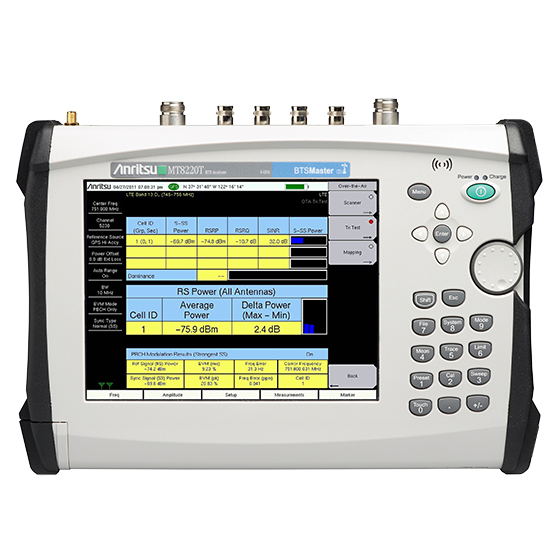
\includegraphics{Imagenes/anritsu1}
\end{figure}

%Cable and Antenna Analyzer
%\begin{itemize}
%	\item 400 MHz to 6 GHz
%	\item Measurements: RL, VSWR, Cable Loss, DTF, Phase (1- and 2-port), Gain
%	\item 2-port gain measurement uncertainty: < 0.45 dB
%	\item 2-port dynamic range: > 100 dB, typical 110 dB (400 MHz to 2800 MHz)
%	\item RF immunity: +17 dBm on-channel, +10 dBm on-frequency
%	\item Calibration: OSL and FlexCal™
%\end{itemize}
%
%Spectrum Analyzer
%\begin{itemize}
%	\item 150 kHz to 7.1 GHz
%	\item Measurements: Occupied Bandwidth, Channel Power, ACPR, C/I, Field Strength, Spectral Emissions, PIM Hunting
%	\item Dynamic range: > 95 dB in 1 Hz RBW
%	\item DANL: –163 dBm in 1 Hz RBW
%	\item Phase noise: –100 dBc/Hz @ 10 kHz offset
%	\item Frequency accuracy: ± 25 ppb with GPS On
%	\item Fast, Performance, No FFT and Burst Detect™ sweep modes
%\end{itemize}

Características
\begin{itemize}
	\item 2-port Cable and Antenna Analyzer 400 MHz to 6 GHz
	\item Spectrum Analyzer 150 kHz to 7.1 GHz
	\item Power Meter 10 MHz to 7.1 GHz
	\item GPS Receiver with Antenna
	\item Bias Tee
	\item High Accuracy Power Meter (up to 26 GHz with external sensor)
	\item Interference Analyzer with Mapping
	\item Channel Scanner
	\item Vector Signal Generator 400 MHz to 6 GHz
	\item Signal Analyzers
	\begin{itemize}
		\item LTE/LTE-A FDD/TDD, NB-IoT, W-CDMA/HSPA+,
		\item GSM/GPRS/EDGE, TD-SCDMA/HSPA+
		\item CDMA, EV-DO
		\item Fixed and Mobile WiMAX
	\end{itemize}
	\item CPRI\footnote{Common Public Radio Interface} RF Analyzer
	\item OBSAI RF Analyzer
	\item BBU Emulation
	\item PIM over CPRI
	\item eMBMS
	\item PIM\footnote{Passive Intermodulation} Alert (a downloadable easyTest™ script)
	\item Standard three-year warranty (battery one-year warranty)
\end{itemize}

\large{\textbf{Precio (desde): U\$D 16000 (usado)}}

\section{R\&S FSH Spectrum Analyzer \cite{fsh}}

The R\&S® FSH is a handheld spectrum analyzer and – depending on the model and the options installed – a power meter, a cable and antenna tester and a two-port vector network analyzer. It provides the most important RF analysis functions that an RF service technician or an installation and maintenance team needs to solve daily routine measurement tasks. For example, it can be used for maintaining or installing transmitter systems, checking cables and antennas, assessing signal quality in broadcasting, radiocommunications and service, measuring electric field strength or in simple lab applications. The R\&S® FSH can perform any of these tasks quickly, reliably and with high measurement accuracy. Weighing only 3 kg, the R\&S® FSH is a handy instrument.

\begin{figure}[H]
	\centering
	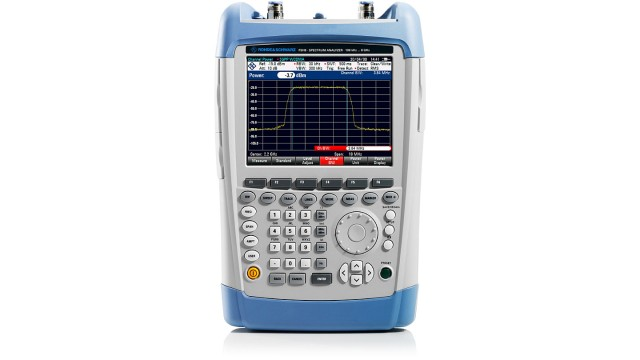
\includegraphics[scale=0.6]{Imagenes/FSH}
\end{figure}

\begin{itemize}
	\item Power measurements on pulsed signals
	\item Channel power measurements
	\item Adjacent channel power measurements
	\item Measurement of spurious emissions (spectrum emission mask)
	\item Measurement of the modulation spectrum on pulsed signals with gated sweep
	\item Analysis of transmit signals (connected to BTS or OTA)
	\begin{itemize}
		\item GSM/GPRS/EDGE
		\item WCDMA/HSDPA/HSPA+
		\item CDMA2000®
		\item 1xEV-DO
		\item LTE FDD/TDD
		\item NB-IoT
		\item TD-SCDMA/HSDPA
	\end{itemize}
	\item Vector network analysis
	\item One-port cable loss measurements
	\item Distance-to-fault measurements
	\item Vector voltmeter
	\item Position finding and increased measurement accuracy using the GPS receiver
\end{itemize}

\large{\textbf{Precio (desde): U\$D 10300}}

\chapter{Diseño de Arquitectura}

\textbf{29/07/2020 - Gino}

\section{Esquemas propuestos}

Los bloques con bordes discontinuos son aquellos opcionales o que no necesariamente deban estar en esa posición.

\subsection{Alternativa 1}

\begin{figure}[H]
	\centering
	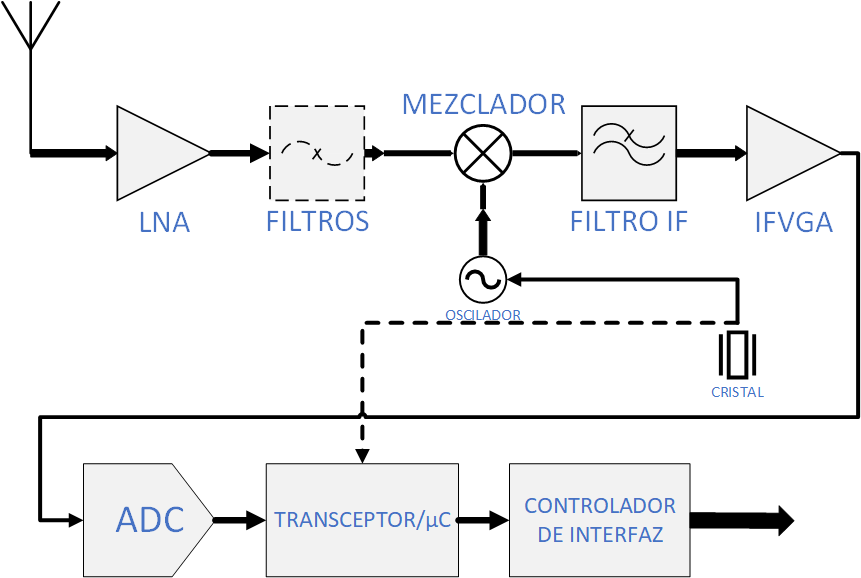
\includegraphics[scale=0.6]{Imagenes/Arquitectura/diagrama1}
\end{figure}

\subsection{Alternativa 2}

Las redes de adaptación pueden no ser necesarias. La más feasible es la segunda, ya que los transceptores suelen tener salidas diferenciales y es preferible tener una con terminación única en algunos casos.

\begin{figure}[H]
	\centering
	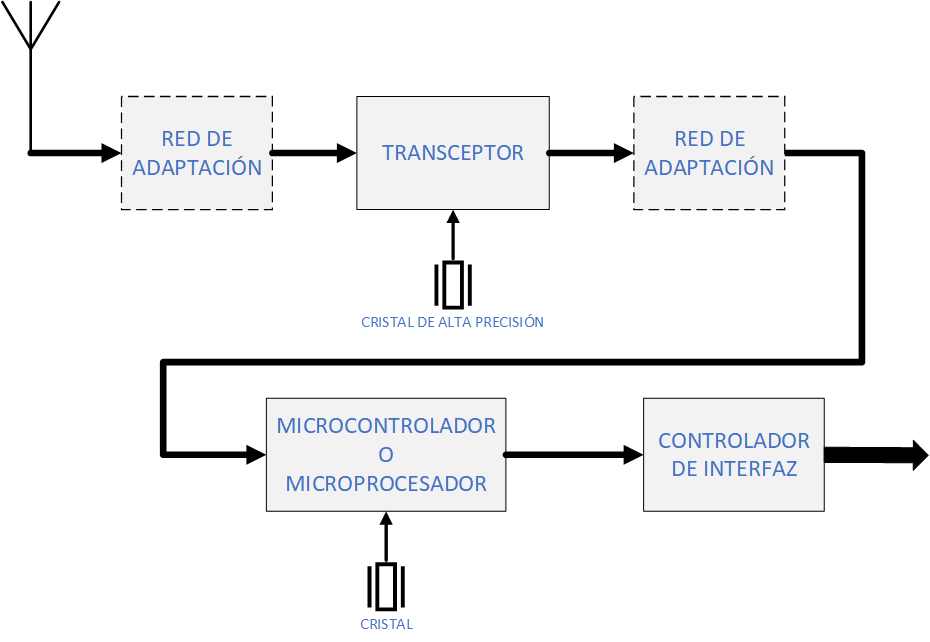
\includegraphics[scale=0.6]{Imagenes/Arquitectura/diagrama2}
\end{figure}

\textbf{03/08/2020 - Gino}
\subsection{Alternativa 3}

Esta bien podría ser la versión final de la arquitectura ya que se contemplan de forma general cada bloque necesario de un diseño típico de hardware SDR. Se supone que todas las interconexiones están adaptadas.

\begin{figure}[H]
	\centering
	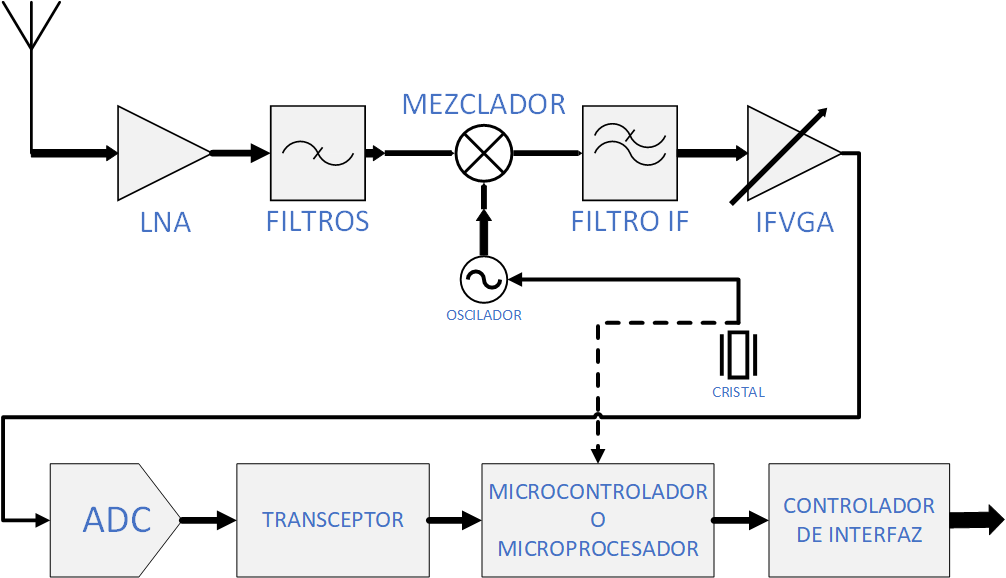
\includegraphics[scale=0.6]{Imagenes/Arquitectura/diagrama3}
\end{figure}

\textbf{29/07/20 Mariano}
\section{Transmisor y Receptor OFDM \cite{tesis}}

Los diagramas de la figura \ref{txrx} son implementaciones analógicas de transmisor y receptor de señales OFDM:

\begin{figure}[H]
	\centering
	\subfigure[Transmisor OFDM]{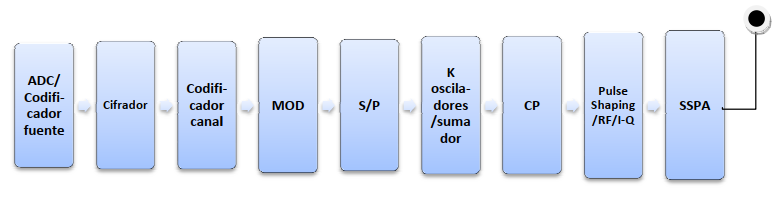
\includegraphics[scale=0.8]{Imagenes/Arquitectura/tx_ofdm} \label{tx_ofdm}}
	\subfigure[Receptor OFDM]{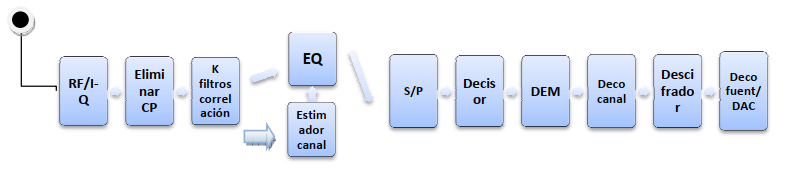
\includegraphics[scale=0.8]{Imagenes/Arquitectura/rx_ofdm}\label{rx_ofdm}}
	\caption{TX y RX OFDM ANALÓGICOS}
	\label{txrx}
\end{figure}

\subsection{Descripción del Transmisor}

\textbf{ADC / Codificador fuente:} Se encarga del muestreo y la cuantificación de la señal proveniente (normalmente) de una fuente adicional.

\textbf{Cifrador:} Incorpora algoritmos que proporcionan algún mecanismo de seguridad para la
comunicación a nivel de la capa física.

\textbf{Codificador de canal:} La codificación del canal se usa para solucionar el problema de requerir altos niveles de potencia de transmisión para lograr tasas de errores bajas. (Mas detalles en \cite{tesis}).

\textbf{Modulador:} Mapea el flujo binario entrante según un esquema de modulación digital convirtiéndolo a la salida en un flujo de símbolos complejos a una tasa $D_{serie}$ símbolos por segundo, o lo que es lo mismo con un tiempo de símbolo $T_{serie}$.

\textbf{Conversor serie/paralelo y Mapeador de subportadoras:} Demultiplexa el flujo de símbolos complejos en  símbolos paralelos haciendo corresponder, a continuación, un símbolo modulado serie a cada subportadora mediante
unas reglas determinadas de mapeo. El subflujo
de símbolos paralelo sale con una tasa $D = D_{serie}/K$ símbolos por segundo (con un
tiempo de símbolo $T = K\cdot T_{serie}$) y se denota mediante $S_{kl}$ , donde $k$ es el subíndice queindica la frecuencia de la subportadora que le corresponde, comprendido entre $k = ±1, ±2, ... , ±K/2$ (la componente DC suele dejarse vacía en sistemas prácticos debidoa motivos de implementación) y $l$ es el subíndice comprendido entre 0 y $L-1$ queindica el instante temporal en la transmisión.

\textbf{Banco de K filtros paso-banda paralelos $+$ sumador:} Esta etapa incorpora los osciladores y aparece solo en la versión analógica. Cada subflujo  a la salida del conversor S/P se hace pasar a través de un filtro
paso-banda. La señal a la salida de cada uno de estos filtros se suma, dando lugar a la señal
OFDM sin prefijo cíclico.
Como se detalla en el esquema digital, los osciladores se implementan mediante la FFT. (Para mas detalles de la versión analógica de este bloque dirigirse a \cite{tesis}).

\textbf{Incorporación del prefijo cíclico:} EL prefijo cíclico es es periodo que se añade entre símbolos para evitar, principalmente, la interferencia ínter-símbolos (ISI). En términos generales consiste en copiar una ultima parte del último símbolo y reproducirlo en este intervalo de guarda, como se ve en la figura \ref{CP}.

\begin{figure}[H]
	\centering
	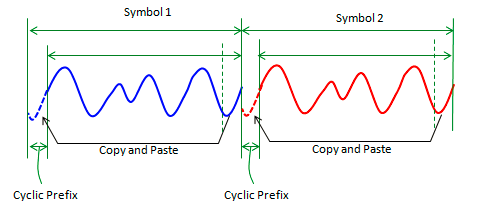
\includegraphics[scale=1]{imagenes/arquitectura/CP}
	\caption{Cyclic Prefix}
	\label{CP}
\end{figure}

Tras el sumador, se añade el prefijo cíclico y como consecuencia la duración del pulso es de $T_s = T + \Delta$. Como efecto no deseado, la incorporación del CP trae consigo una reducción de la eficiencia energetica y la tasa binaria transmitida.

\textbf{Oscilador RF y modulador IQ:} Consiste en un oscilador VCO o PLL que proporciona la portadora de la señal OFDM a frecuencia de UHF. Para que no haya una disminución de la SNR es muy importante que el oscilador en el transmisor y en le receptor estén sincronizados.

La portadora en fase se desfasa 90° obteniéndose la portadora en cuadratura. Ambas son multiplicadas respectivamente por la parte real e imaginaria de la señal OFDM.

\textbf{Amplificador de potencia:} Encargado de la amplificación de la señal para ser alimentada a la antena o a las L antenas.

\subsection{Descripción del Receptor} %Revisar conceptos

La señal recibida por la antena es bajada en frecuencia por un oscilador local que debe estar lo más adaptado posible al oscilador del transmisor. Aun así, los errores causados por desplazamiento en frecuencia y ruido de fase deben ser corregidos mediante técnicas de sincronización en frecuencia.





%--------------------------------
Como esta implementación (analógica) es costosa y un poco engorrosa se opta por una alternativa basada en el cálculo de la transformada discreta de Fourier mediante el algoritmo de la transformada Rápida de Fourier cuya eficiencia y facilidad de implementación fue la que permitió el éxito de OFDM. Esta alternativa digital se ve en la figura \ref{alt_dig}.

\begin{figure}[H]
	\centering
	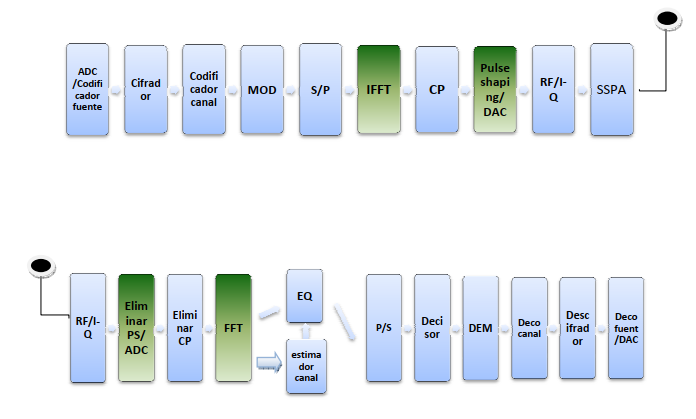
\includegraphics[scale=0.9]{Imagenes/Arquitectura/alt_dig}
	\caption{TX y RX OFDM DIGITALES}
	\label{alt_dig}
\end{figure}

En la figura \ref{alt_dig} los bloques en verde indican los cambios respecto al TX y RX analógico.


\chapter{Elección de componentes de cada bloque de la arquitectura}

\textbf{04/08/20 Mariano}

\section{Aspectos generales} \cite{sdr_engineers}

En lineas generales un SDR está conformado por las siguientes secciones:

\begin{itemize}
	\item Una sección analógica de RF (antena, filtros RF, multiplexores, LNA, atenuadores, mezcladores).
	\item Una sección analógica de Banda base (filtros analógicos, ADS y/o DAC).
	\item Unidades de procesamiento de señal (Filtros dentro del transceptor, FPGA o DSP, o procesadores de propósitos generales).
\end{itemize}

Para tener una referencia observamos el caso de PLUTO SDR. Las secciones anteriores, en esta plataforma especifica se ven conformadas por lo siguiente:

\begin{itemize}
	\item Una sección analógica de RF (antena, filtros RF, multiplexores, LNA, atenuadores, mezcladores)
		\subitem Antena y filtros de RF son responsabilidad del usuario.
		\subitem Los demás items (multiplexores, LNAs, atenuadores y mezcladores) están integrados en el transceptor AD9363.
		
	\item Una sección analógica de Banda base (filtros analógicos, ADS y/o DAC).
		\subitem Toda esta sección está implementada dentro del transceptor nombrado anteriormente.
		 
	\item Unidades de procesamiento de señal (Filtros dentro del transceptor, FPGA o DSP, o procesadores de propósitos generales). Esta sección se divide entre lo siguiente:
		\subitem Una parte es implementada en el AD9363. Esto  incluye los filtros de interpolación y diezmado de la banda media y los filtros FIR programables de 128 taps.
		\subitem Filtrados y diezmados opcionales se hacen con la FPGA Xilinx Zynq.
		\subitem La información I/Q pasa por el USB al host y de ahí se puede continuar procesándola con MATLAB.
\end{itemize}

\textbf{05/08/20 Gino}
\section{Transceptor}

\subsection{LMS6002D}

\url{https://limemicro.com/technology/lms6002d/}

Transceptor de Lime Microsystems con bajo costo (alrededor de \textbf{35 dólares}) dadas las prestaciones y comparado con otros integrados en el mismo segmento. 

\begin{itemize}
	\item Single chip transceiver
	\item Covers 300MHz to 3.8GHz
	\item Fully differential baseband signals
	\item Few external components
	\item Programmable modulation bandwidth: 1.5, 1.75, 2.5, 2.75, 3, 3.84, 5, 5.5, 6, 7, 8.75, 10, 12, 14, 20 and 28MHz
	\item Supports both FDD and TDD full duplex
	\item Integrated high performance 12-bit ADC and DAC
	\item Low voltage operation, 1.8V and 3.3V
	\item Standby current less than 1mA
	\item Tx RF output +6dBm, continuous wave
	\item 120 pin DQFN package
	\item Provision for Full Calibration
	\item Power down
	\item Serial interface
\end{itemize}

\subsection{AD9363}

\url{ttps://www.analog.com/en/products/ad9363.html#product-overview}

Transceptor de Analog Devices de costo medio (entre \textbf{60 y 120 dólares}). 

\begin{itemize}
	\item Radio frequency (RF) 2 × 2 transceiver with integrated 12-bit DACs and ADCs
	\item Wide bandwidth: 325 MHz to 3.8 GHz
	\item Supports time division duplex (TDD) and frequency division duplex (FDD) operation
	\item Tunable channel bandwidth (BW): up to 20 MHz
	\item Receivers: 6 differential or 12 single-ended inputs
	\item Superior receiver sensitivity with a noise figure: 3 dB
	\item Receive (Rx) gain control
	\begin{itemize}
		\item Real-time monitor and control signals for manual gain
		\item Independent automatic gain control (AGC)
	\end{itemize}
	\item Dual transmitters: 4 differential outputs
	\item Highly linear broadband transmitter
	\begin{itemize}
		\item Transmit (Tx) error vector magnitude (EVM): -34 dB
		\item Tx noise: $\leqslant-$157 dBm/Hz noise floor
		\item Tx monitor: 66 dB dynamic range with 1 dB accuracy
	\end{itemize}
	\item Integrated fractional N synthesizers
	\item 2.4 Hz local oscillator (LO) step size
	\item CMOS/LVDS digital interface
\end{itemize}

\subsection{NRF9160}

\url{https://www.nordicsemi.com/Products/Low-power-cellular-IoT/nRF9160}

Transceptor de Nordic Semiconductor. Tiene un costo bajo (\textbf{25 dólares} aproximadamente). La desventaja es que está diseñado para NB-IoT por ende los ancho de banda soportados son de 200 kHz y 1.4 MHz. Además, solo soporta frecuencias de entrada hasta los 2200 MHz, por lo que la banda 7 quedaría fuera. Lo bueno es que trae integrado un procesador Arm Cortex-M33 y existe software dedicado a monitoreo de enlaces LTE (\url{https://www.youtube.com/watch?v=m5V4Vo_Xemk})

\chapter{Varios}

\textbf{10/09/20 Gino}
\begin{itemize}
	\item Reunión con Ing. Riva y Zerbini para definición de arquitectura.
	\item Solicitud de muestras gratis a Maxim (MAX2837, MAX5864).
\end{itemize}
\textbf{17/09/20 Gino}
\begin{itemize}
	\item Solicitud de muestra gratis a Qorvo (RFFC5071).
	\begin{figure}[H]
		\centering
		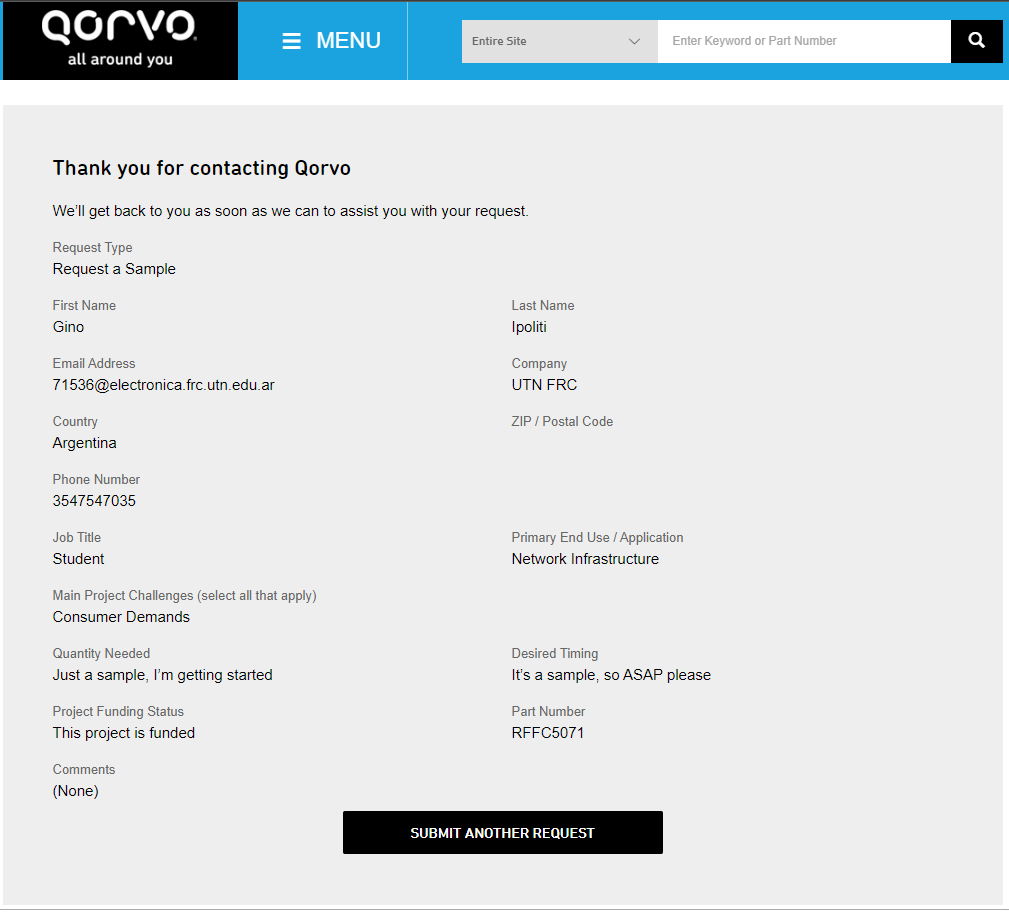
\includegraphics[scale=0.6]{Imagenes/sample_qorvo}
		\caption{Solicitud de sample}
	\end{figure}
\end{itemize}

\chapter{Esquemático}

\section{Frontend RF}
\subsection{Notas de diseño}

\textbf{30/12/2020 Gino}
\begin{itemize}
	\item En vez de usar un balun 4:1 como sugiere el fabricante en el datasheet, se opta por usar uno 1:1 y 2 chokes de RF, siendo una alternativa equivalente.
\end{itemize}

\bibliographystyle{IEEEtran}	
\bibliography{bibliografia}
\nocite{*}
\end{document}